% This is the TEST file in the Figures folder.  

\documentclass[11pt]{amsart}
\usepackage{geometry}                % See geometry.pdf to learn the layout options. There are lots.
\geometry{letterpaper}                   % ... or a4paper or a5paper or ... 
%\geometry{landscape}                % Activate for for rotated page geometry
%\usepackage[parfill]{parskip}    % Activate to begin paragraphs with an empty line rather than an indent
\usepackage{graphicx}
\usepackage{amssymb}
\usepackage{epstopdf}
\DeclareGraphicsRule{.tif}{png}{.png}{`convert #1 `dirname #1`/`basename #1 .tif`.png}


\usepackage{tikz}
\usetikzlibrary{shapes.geometric}
\usepackage{pgfplots}
\pgfplotsset{compat=newest} 
\usepackage{bytefield}


\title{ \vspace{-80pt} Testing the Ethernet Figures }
\author{Test of Ethernet Figures in this folder}
%\date{}                                           % Activate to display a given date or no date

\begin{document}

\maketitle
\vspace{-20pt}

\begin{figure}[h!]. \centering  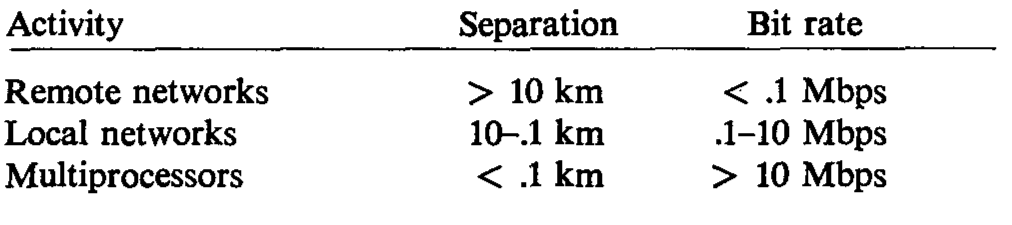
\includegraphics[trim =0mm 0mm 0mm 0mm, clip, width=10cm]{Ethernet-Table-0.png}    \caption{Ethernet Table 0} \end{figure}

%!TEX root =../Metcalfe+Boggs.tex
%!TEX TS-program XeLaTeX
% This is what ChatGPT came up with for Table 1 3 in the Metcalfe + Boggs Paper

\vspace{-5pt} 
\begin{table}[ht]
\centering \tiny  %\small
\begin{tabular}{l l l}
\hline
\textbf{Activity} & \textbf{Separation} & \textbf{Bit rate} \\
%\hline
Remote networks   & $> 10$ km  & $< 0.1$ Mbps  \\
Local networks    & $10\text{--}1$ km & $0.1\text{--}10$ Mbps \\
Multiprocessors   & $< 1$ km   & $> 10$ Mbps   \\
\hline
\end{tabular}
%\vspace{10pt}
%\caption{Comparison of network activities by separation and bit rate}
\label{tab:network_comparison}
\end{table}
\vspace{-8pt} 

\section*{FIGURE 1} 

\newpage

\begin{figure}[h!]. \centering  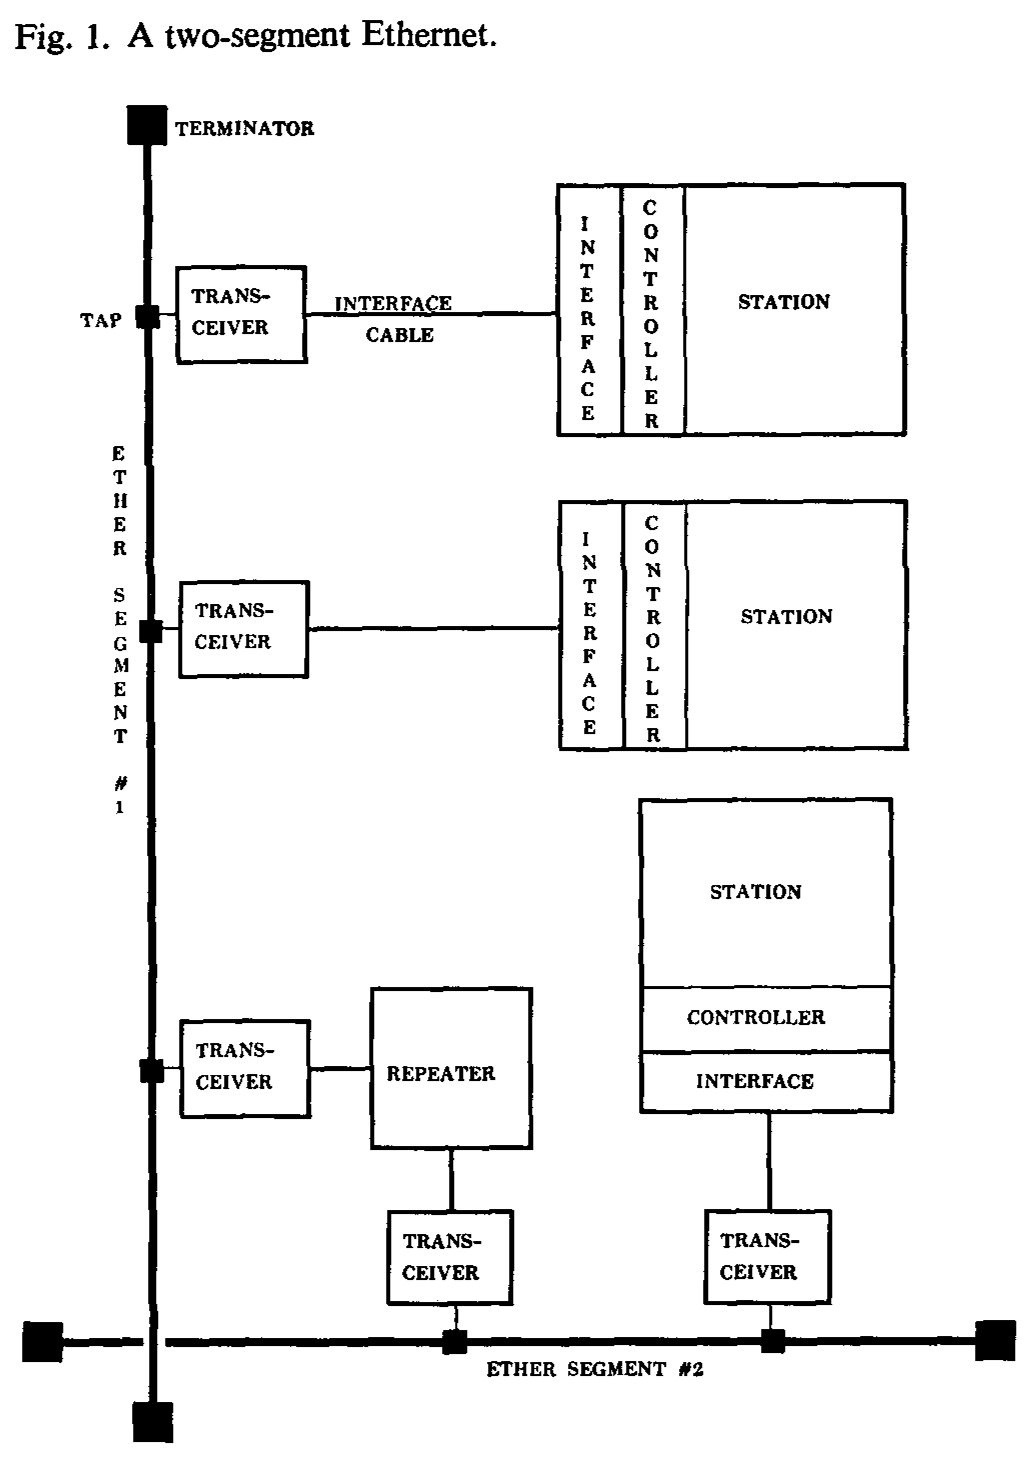
\includegraphics[trim =0mm 0mm 0mm 0mm, clip, width=6cm]{Ethernet-Fig-1.png}    \caption{Ethernet Fig-1 PNG} \end{figure}

% This is what ChatGPT came up with for Figure 1 in the Metcalfe + Boggs Paper

% A rough approximation of "Fig. 1. A two-segment Ethernet."
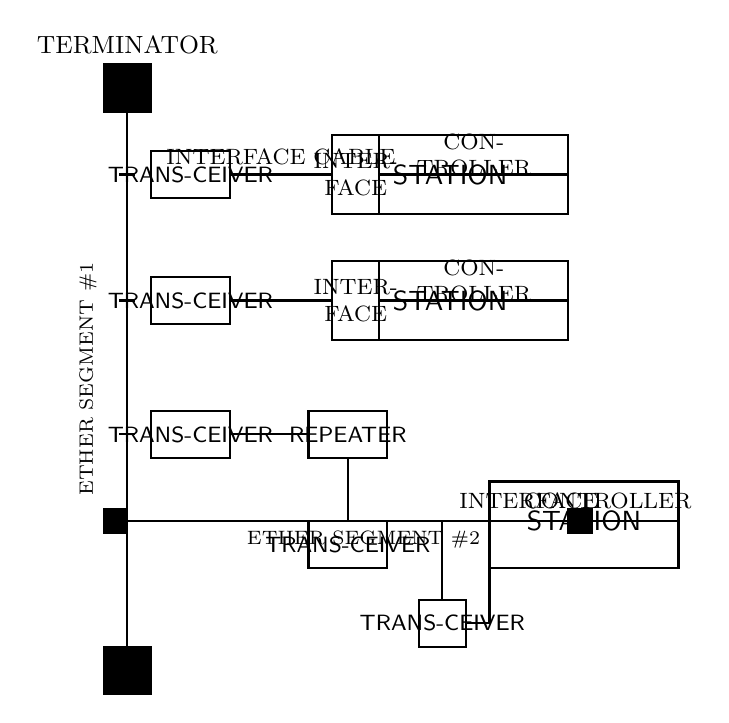
\begin{tikzpicture}[font=\sffamily, line width=0.8pt]
    %----------------------
    % ETHER SEGMENT #1 (vertical)
    %----------------------
    % Draw top terminator
    \filldraw[black] (-0.3,8) rectangle (0.3,7.4);
    \node[above, font=\small] at (0,8) {TERMINATOR};

    % Draw vertical cable
    \draw (0,7.4) -- (0,0.6);

    % Label the vertical cable
    \node[rotate=90, font=\scriptsize] at (-0.5,4) {ETHER SEGMENT \#1};

    % Draw bottom terminator on segment #1
    \filldraw[black] (-0.3,0.6) rectangle (0.3,0.0);

    %----------------------
    % FIRST TRANSCEIVER + STATION
    %----------------------
    % The transceiver "tap" at around y=6.6
    \draw[thick] (-0.1,6.6) -- (0.1,6.6);
    \draw[rectangle, fill=white] (0.3,6.9) rectangle (1.3,6.3);
    \node at (0.8,6.6) {\footnotesize TRANS-\\CEIVER};

    % Cable to station (interface,controller,station)
    \draw (1.3,6.6) -- (2.6,6.6);
    \node[above, font=\footnotesize] at (1.95,6.6) {INTERFACE CABLE};

    % Station block (Interface, Controller, Station)
    % We'll stack small rectangles
    % Outer "station" box at (2.6,6.6) + 4 cm width
    \draw (2.6,7.1) rectangle (5.6,6.1);  % large station box
    \node at (4.1,6.6) {STATION};
    % Put a narrow interface/controller label block on left
    \draw (2.6,7.1) -- (3.2,7.1) -- (3.2,6.1) -- (2.6,6.1) -- cycle;
    % Sub-boxes for interface, controller
    \node[align=center, font=\footnotesize] at (2.9,6.6) {INTER-\\FACE};
    \draw (3.2,7.1) -- (3.2,6.1);

    \draw (3.2,6.6) -- (5.6,6.6);

    \node[align=center, font=\footnotesize] at (4.4,6.85) {CON-\\TROLLER};

    %----------------------
    % SECOND TRANSCEIVER + STATION
    %----------------------
    % Another tap at y=5.0
    \draw[thick] (-0.1,5.0) -- (0.1,5.0);
    \draw (0.3,5.3) rectangle (1.3,4.7);
    \node at (0.8,5.0) {\footnotesize TRANS-\\CEIVER};

    % Cable to second station
    \draw (1.3,5.0) -- (2.6,5.0);

    % Second station block
    \draw (2.6,5.5) rectangle (5.6,4.5);
    \node at (4.1,5.0) {STATION};
    % Left label region
    \draw (2.6,5.5) -- (3.2,5.5) -- (3.2,4.5) -- (2.6,4.5) -- cycle;
    \node[font=\footnotesize, align=center] at (2.9,5.0) {INTER-\\FACE};
    \draw (3.2,5.0) -- (5.6,5.0);
    \node[font=\footnotesize, align=center] at (4.4,5.25) {CON-\\TROLLER};

    %----------------------
    % REPEATER + bridging to ETHER SEGMENT #2 (horizontal)
    %----------------------
    % Tap at y=3.3 for the transceiver
    \draw[thick] (-0.1,3.3) -- (0.1,3.3);
    \draw (0.3,3.6) rectangle (1.3,3.0);
    \node at (0.8,3.3) {\footnotesize TRANS-\\CEIVER};

    % Repeater to transceiver below it
    \draw (1.3,3.3) -- (2.3,3.3);
    \draw (2.3,3.6) rectangle (3.3,3.0);
    \node at (2.8,3.3) {\footnotesize REPEATER};

    \draw (2.8,3.0) -- (2.8,2.2);
    \draw (2.3,2.2) rectangle (3.3,1.6);
    \node at (2.8,1.9) {\footnotesize TRANS-\\CEIVER};

    % Horizontal Ether Segment #2
    \draw (0,2.2) -- (5.6,2.2); % connect from vertical cable to the next cable
    % A black square 'junction'
    \filldraw[black] (-0.3,2.35) rectangle (0,2.05);

    % Label horizontal cable
    \node[below, font=\scriptsize] at (3,2.2) {ETHER SEGMENT \#2};

    % Terminator on the far right
    \filldraw[black] (5.6,2.35) rectangle (5.9,2.05);

    %----------------------
    % Station on ETHER SEGMENT #2
    %----------------------
    % A transceiver connected to the station
    \draw[thick] (4,2.2) -- (4,1.2);
    \draw (3.7,1.2) rectangle (4.3,0.6);
    \node at (4,0.9) {\footnotesize TRANS-\\CEIVER};

    % Station block above
    \draw (4.6,2.7) rectangle (7.0,1.6); 
    \node at (5.8,2.2) {STATION};
    % interface, controller boxes stacked
    \draw (4.6,2.2) -- (7.0,2.2);
    \draw (4.6,1.6) -- (7.0,1.6);
    \node[font=\footnotesize] at (5.1,2.45) {INTERFACE};
    \node[font=\footnotesize] at (6.1,2.45) {CONTROLLER};

    % Cable from transceiver into the station
    \draw (4.3,0.9) -- (4.6,0.9) -- (4.6,1.6);

\end{tikzpicture}

 

\newpage
\section*{FIGURE 2} 

\begin{figure}[h!]. \centering  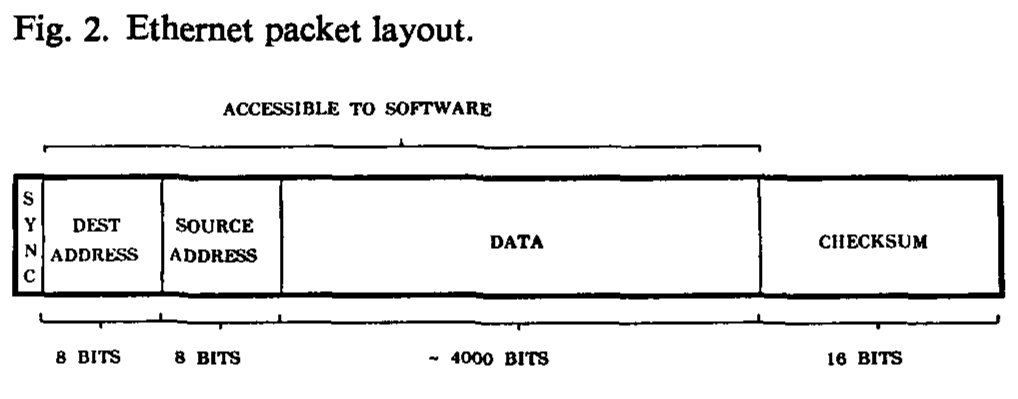
\includegraphics[trim =0mm 0mm 0mm 0mm, clip, width=6cm]{Ethernet-Fig-2.png}    \caption{Ethernet Fig-2 PNG} \end{figure}

%!TEX root =Test-Ethernet-Figures.tex
% This is what ChatGPT came up with  
\begin{figure}[ht]
\centering
% Make boxes wider by increasing bitwidth; reduce text size by \scriptsize
{\scriptsize
  \begin{bytefield}[bitwidth=2em]{32}
    \bitheader{0-7,8-15,16-23,24-31} \\
    \bitbox{8}{\textbf{SYNC}} &
    \bitbox{8}{\textbf{Dest.\ Addr.}} &
    \bitbox{8}{\textbf{Source Addr.}} &
    \bitbox{8}{\textbf{Type/Len}}
  \end{bytefield}

  \vspace{0.5em}

  \begin{bytefield}[bitwidth=2em]{32}
    \bitheader{0-31} \\
    \bitbox{32}{\textbf{Data (4000 bits total)}}
  \end{bytefield}

  \vspace{0.5em}

  \begin{bytefield}[bitwidth=2em]{16}
    \bitheader{0-15}\\
    \bitbox{16}{\textbf{Checksum}}
  \end{bytefield}
}
\caption{Ethernet packet layout with wider boxes and smaller text.}
\end{figure}

% 
% This is what ChatGPT came up with for Figure 2 in the Metcalfe + Boggs Paper

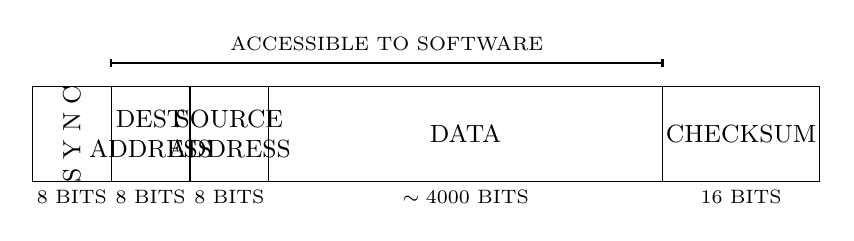
\begin{tikzpicture}[font=\sffamily] %, thick]

% Overall height of the boxes:
\def\boxheight{1.2}
% Vertical offset (so we can place bit labels below):
\def\yoffset{0.0}

%--- Define horizontal widths (approximate) ---
% Sync: 1 cm, Dest: 1 cm, Source: 1 cm, Data: 5 cm, Checksum: 2 cm
\def\xSync{1}
\def\xDest{1}
\def\xSource{1}
\def\xData{5}
\def\xChecksum{2}
% We will draw them in one line from x=0 up to x=totalWidth
\pgfmathsetmacro{\xTotal}{\xSync + \xDest + \xSource + \xData + \xChecksum}

%--- Draw main outer rectangle (from x=0 to x=\xTotal, y=\yoffset up to y=\yoffset+\boxheight)
\draw (0,\yoffset) rectangle (\xTotal,{\yoffset+\boxheight});

%--- Vertical dividing lines and labels ---
% 1) SYNC boundary at x= \xSync
\draw (\xSync,\yoffset) -- (\xSync,{\yoffset+\boxheight});
% 2) DEST boundary at x= \xSync + \xDest
\pgfmathsetmacro{\xDestBound}{\xSync + \xDest}
\draw (\xDestBound,\yoffset) -- (\xDestBound,{\yoffset+\boxheight});
% 3) SOURCE boundary at x= \xDestBound + \xSource
\pgfmathsetmacro{\xSourceBound}{\xDestBound + \xSource}
\draw (\xSourceBound,\yoffset) -- (\xSourceBound,{\yoffset+\boxheight});
% 4) DATA boundary at x= \xSourceBound + \xData
\pgfmathsetmacro{\xDataBound}{\xSourceBound + \xData}
\draw (\xDataBound,\yoffset) -- (\xDataBound,{\yoffset+\boxheight});

%--- Labels INSIDE the boxes ---
% SYNC (rotated to match figure’s style)
\node[rotate=90, font=\small] at (0.5*\xSync, \yoffset+0.5*\boxheight) {S Y N C};
% DEST ADDRESS
\node[align=center, font=\small] at (\xSync + 0.5*\xDest, \yoffset+0.5*\boxheight) {DEST\\ADDRESS};
% SOURCE ADDRESS
\node[align=center, font=\small] at (\xDestBound + 0.5*\xSource, \yoffset+0.5*\boxheight) {SOURCE\\ADDRESS};
% DATA
\node[font=\small] at (\xSourceBound + 0.5*\xData, \yoffset+0.5*\boxheight) {DATA};
% CHECKSUM
\node[font=\small] at (\xDataBound + 0.5*\xChecksum, \yoffset+0.5*\boxheight) {CHECKSUM};

%--- Bit-size labels below ---
\node[font=\scriptsize] at (0.5*\xSync, \yoffset-0.2) {8 BITS};
\node[font=\scriptsize] at (\xSync + 0.5*\xDest, \yoffset-0.2) {8 BITS};
\node[font=\scriptsize] at (\xDestBound + 0.5*\xSource, \yoffset-0.2) {8 BITS};
\node[font=\scriptsize] at (\xSourceBound + 0.5*\xData, \yoffset-0.2) {$\sim 4000$ BITS};
\node[font=\scriptsize] at (\xDataBound + 0.5*\xChecksum, \yoffset-0.2) {16 BITS};

%--- Bracket for "ACCESSIBLE TO SOFTWARE" above the top 
%    (spans from the DEST boundary to the DATA boundary)
\draw[thick] (\xSync,{\yoffset+\boxheight+0.3}) -- (\xDataBound,{\yoffset+\boxheight+0.3});
\draw[thick] (\xSync,{\yoffset+\boxheight+0.25}) -- (\xSync,{\yoffset+\boxheight+0.35});
\draw[thick] (\xDataBound,{\yoffset+\boxheight+0.25}) -- (\xDataBound,{\yoffset+\boxheight+0.35});

\node[font=\scriptsize] at (0.5*\xSync+0.5*\xDataBound,{\yoffset+\boxheight+0.55}) {ACCESSIBLE TO SOFTWARE};

\end{tikzpicture}

 

\newpage
\section*{FIGURE 3} 

\begin{figure}[h!]. \centering  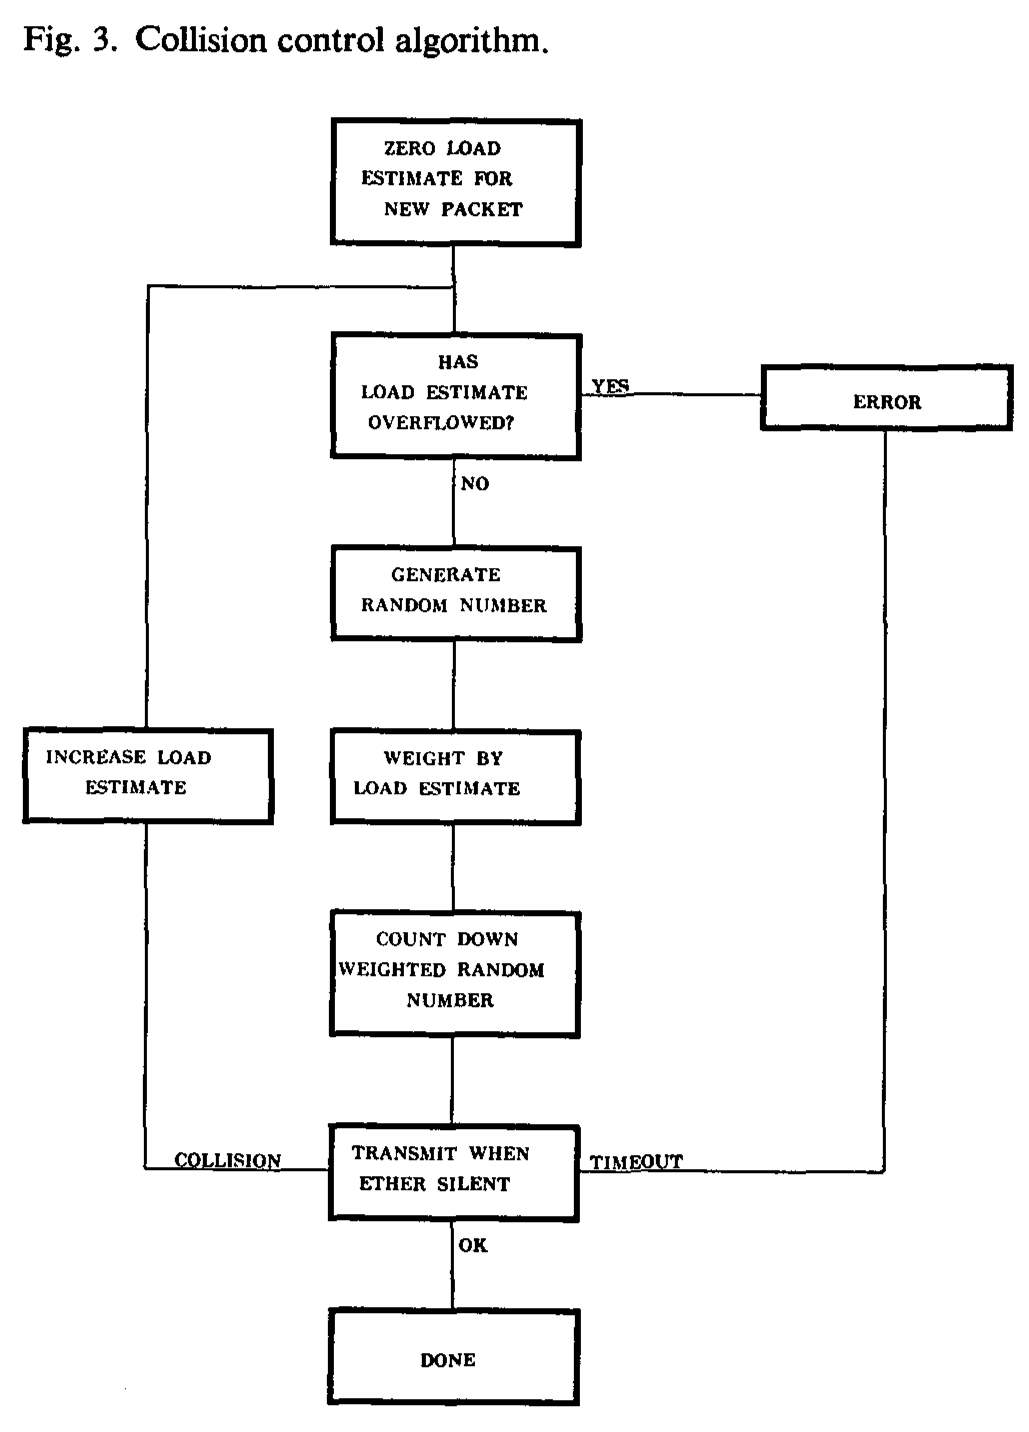
\includegraphics[trim =0mm 0mm 0mm 0mm, clip, width=8cm]{Ethernet-Fig-3.png}    \caption{Ethernet-Fig-3.png} \end{figure}

% This is what ChatGPT came up with for Figure 3 in the Metcalfe + Boggs Paper
%\begin{center}
%\begin{tikzpicture}[
%    node distance=2cm,
%    % A couple of convenient style aliases:
%    block/.style = {rectangle, draw, rounded corners, align=center, minimum width=3cm, minimum height=1cm},
%    decision/.style = {diamond, draw, aspect=2, align=center, inner sep=0pt},
%    line/.style = {->, thick}
%]
%
%% --- NODES ---
%\node[block]               (init) {Zero load\\estimate for new packet};
%\node[decision, below of=init] (overflow) {Has load\\estimate overflowed?};
%\node[block, right of=overflow, xshift=3cm] (error) {Error};
%\node[block, below of=overflow]    (rand) {Generate\\random number};
%\node[block, below of=rand]        (weight) {Weight by\\load estimate};
%\node[block, below of=weight]      (count) {Count down\\weighted random number};
%\node[block, below of=count]       (transmit) {Transmit when\\ether silent};
%\node[block, below of=transmit]    (done) {Done};
%
%% For the “Increase load estimate” block on the left,
%% we place it relative to (rand). 
%\node[block, left of=rand, xshift=-3cm] (increase) {Increase\\load estimate};
%
%% --- ARROWS ---
%% Straight down path
%\draw [line] (init) -- (overflow);
%\draw [line] (overflow) -- node [near start, anchor=west] {No} (rand);
%\draw [line] (rand) -- (weight);
%\draw [line] (weight) -- (count);
%\draw [line] (count) -- (transmit);
%\draw [line] (transmit) -- node [midway, right] {OK} (done);
%
%% Overflow -> Error
%\draw [line] (overflow) -- node [near start, anchor=south] {Yes} (error);
%
%% Increase load estimate arrow
%\draw [line] (increase) |- (rand);
%
%% Extra collision/timeout arrows from “Transmit” if you need them:
%%\draw [line] (transmit) -| node [near start, above] {Collision} (increase);
%%\draw [line] (transmit) -| node [near start, below] {Timeout} (error);
%
%\end{tikzpicture}
%\end{center}

%\begin{figure}[ht]
%\centering
%\begin{tikzpicture}[
%    node distance=2.2cm,  % controls vertical/horizontal spacing
%    font=\small,
%    % Styles for nodes:
%    block/.style   ={rectangle, draw, rounded corners, align=center, 
%                     minimum width=3cm, minimum height=1cm},
%    decision/.style={diamond, draw, aspect=2, align=center, inner sep=0pt},
%    % Style for arrows:
%    line/.style    ={->, thick},
%]
%
%% --- NODES ---
%\node[block]                (init)    {Zero load estimate\\for new packet};
%\node[decision, below of=init] (overflow) {Has load estimate\\overflowed?};
%\node[block, right of=overflow, xshift=3cm] (error) {Error};
%\node[block, below of=overflow] (rand) {Generate\\random number};
%\node[block, below of=rand]   (weight) {Weight by\\load estimate};
%\node[block, below of=weight] (count)  {Count down\\weighted random number};
%\node[block, below of=count]  (transmit) {Transmit when\\ether silent};
%\node[block, below of=transmit] (done) {Done};
%
%% "Increase load estimate" is off to the left of the decision node:
%\node[block, left of=overflow, xshift=-3.5cm] (increase) {Increase\\load estimate};
%
%% --- ARROWS ---
%% Top-down main flow
%\draw[line] (init) -- (overflow);
%\draw[line] (overflow) -- node[midway, anchor=west] {No} (rand);
%\draw[line] (rand) -- (weight);
%\draw[line] (weight) -- (count);
%\draw[line] (count) -- (transmit);
%\draw[line] (transmit) -- node[midway, anchor=west] {OK} (done);
%
%% Overflow -> Error
%\draw[line] (overflow) -- node[midway, anchor=south] {Yes} (error);
%
%% Transmit -> Increase load estimate (Collision)
%\draw[line] (transmit) -| node[pos=0.25, above] {Collision} (increase);
%
%% Increase load estimate -> Overflow decision
%\draw[line] (increase) -- (overflow);
%
%% Transmit -> Error (Timeout)
%\draw[line] (transmit) -- node[midway, anchor=east] {Timeout} (error);
%
%\end{tikzpicture}
%\caption{Collision Control Algorithm Flowchart}
%\label{fig:collision-control}
%\end{figure}

%\begin{figure}[ht]
%\centering
%\begin{tikzpicture}[
%    node distance=2.2cm,    % controls spacing
%    font=\small,           % slightly smaller text
%    % Node styles:
%    block/.style={rectangle, draw, rounded corners, align=center,
%                  minimum width=3cm, minimum height=1cm},
%    decision/.style={diamond, draw, aspect=2, align=center, inner sep=0pt},
%    % Arrow style:
%    line/.style={->, thick}
%]
%
%% --- NODES (ALL-CAPS TEXT) ---
%\node[block]                   (init)    {ZERO LOAD ESTIMATE\\FOR NEW PACKET};
%\node[decision, below of=init] (overflow){HAS LOAD ESTIMATE\\OVERFLOWED?};
%\node[block, right of=overflow, xshift=3cm] (error)   {ERROR};
%\node[block, below of=overflow] (rand)   {GENERATE RANDOM NUMBER};
%\node[block, below of=rand]   (weight)   {WEIGHT BY LOAD ESTIMATE};
%\node[block, below of=weight] (count)    {COUNT DOWN\\WEIGHTED RANDOM NUMBER};
%\node[block, below of=count]  (transmit) {TRANSMIT WHEN\\ETHER SILENT};
%\node[block, below of=transmit] (done)   {DONE};
%
%% "INCREASE LOAD ESTIMATE" on the left
%\node[block, left of=overflow, xshift=-3.5cm] (increase)
%      {INCREASE LOAD\\ESTIMATE};
%
%% --- ARROWS ---
%% Main top-down path
%\draw[line] (init) -- (overflow);
%\draw[line] (overflow) -- node[midway, anchor=west] {NO} (rand);
%\draw[line] (rand) -- (weight);
%\draw[line] (weight) -- (count);
%\draw[line] (count) -- (transmit);
%\draw[line] (transmit) -- node[midway, anchor=west] {OK} (done);
%
%% Overflow -> Error
%\draw[line] (overflow) -- node[midway, anchor=south] {YES} (error);
%
%% Collision path: arrow from transmit to increase load (L-shaped)
%\draw[line] (transmit.west) -| node[pos=0.25, anchor=south] {COLLISION} (increase.south);
%
%% Increase load -> back to Overflow
%\draw[line] (increase) -- (overflow);
%
%% Timeout path: arrow from transmit to error (L-shaped, goes right then up)
%\draw[line] (transmit.east) -- ++(1.5,0) |- node[pos=0.25, anchor=south] {TIMEOUT} (error.south);
%
%\end{tikzpicture}
%\caption{Collision Control Algorithm Flowchart (All-Caps Text)}
%\end{figure}

\begin{figure}[ht]
\centering
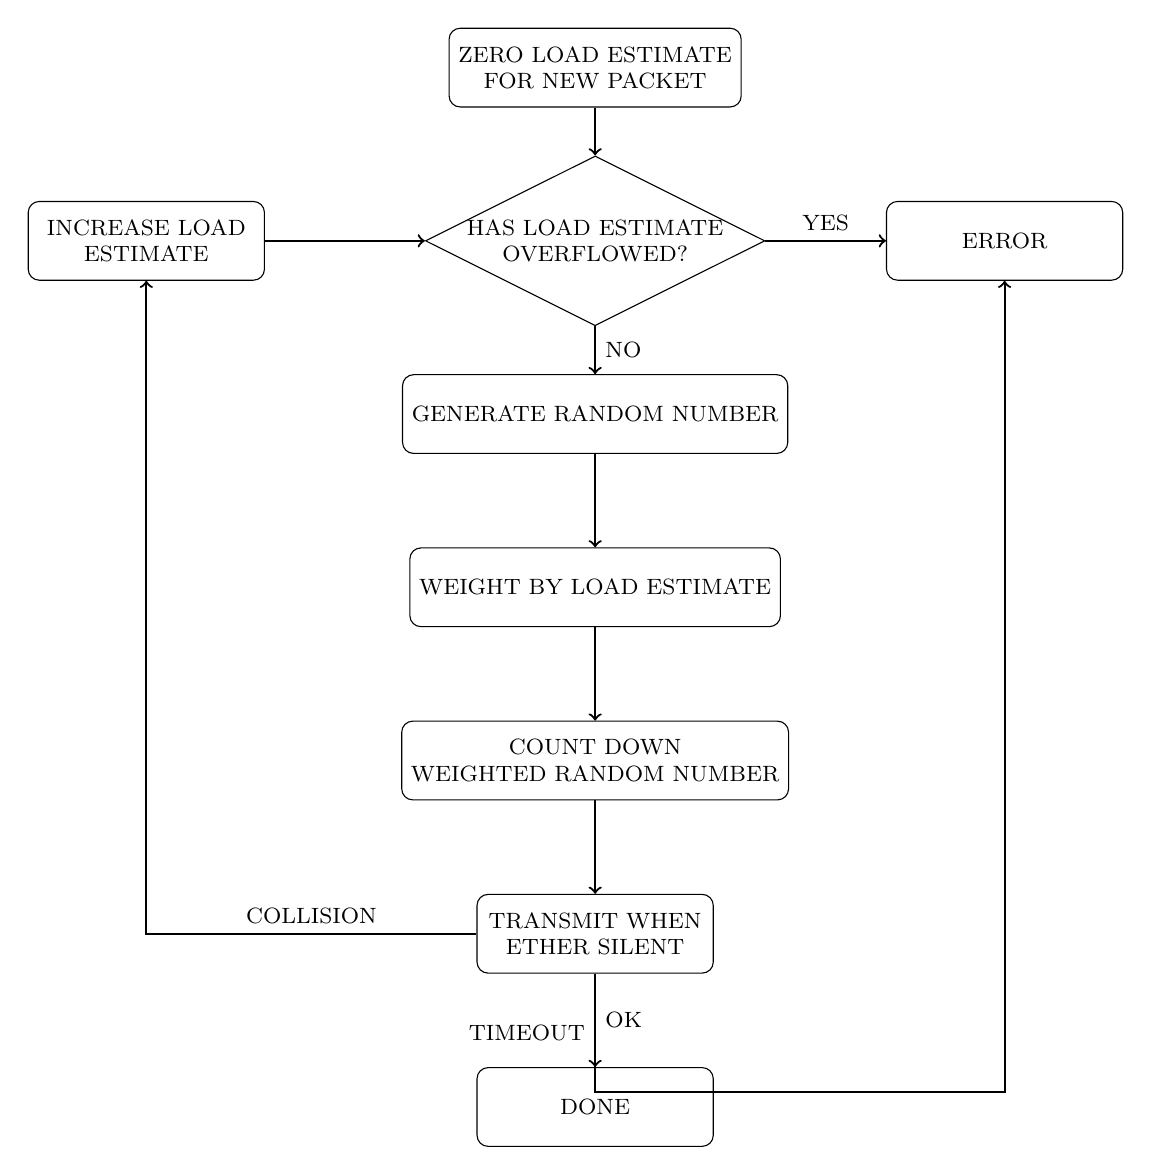
\begin{tikzpicture}[
    node distance=2.2cm,
    font=\footnotesize,  % One size smaller than normal
    % Node styles:
    block/.style={rectangle, draw, rounded corners, align=center,
                  minimum width=3cm, minimum height=1cm},
    decision/.style={diamond, draw, aspect=2, align=center, inner sep=0pt},
    % Arrow style:
    line/.style={->, thick},
]
% --- NODES (ALL CAPS) ---
\node[block]                  (init)    {ZERO LOAD ESTIMATE\\FOR NEW PACKET};
\node[decision, below of=init](overflow){HAS LOAD ESTIMATE\\OVERFLOWED?};
\node[block, right of=overflow, xshift=3cm] (error) {ERROR};
\node[block, below of=overflow] (rand)   {GENERATE RANDOM NUMBER};
\node[block, below of=rand]   (weight)   {WEIGHT BY LOAD ESTIMATE};
\node[block, below of=weight] (count)    {COUNT DOWN\\WEIGHTED RANDOM NUMBER};
\node[block, below of=count]  (transmit) {TRANSMIT WHEN\\ETHER SILENT};
\node[block, below of=transmit] (done)   {DONE};

% "INCREASE LOAD ESTIMATE" on the left
\node[block, left of=overflow, xshift=-3.5cm] (increase)
      {INCREASE LOAD\\ESTIMATE};

% --- ARROWS ---
% Main top-down path
\draw[line] (init) -- (overflow);
\draw[line] (overflow) -- node[midway, anchor=west] {NO} (rand);
\draw[line] (rand) -- (weight);
\draw[line] (weight) -- (count);
\draw[line] (count) -- (transmit);
\draw[line] (transmit) -- node[midway, anchor=west] {OK} (done);

% Overflow -> Error
\draw[line] (overflow) -- node[midway, anchor=south] {YES} (error);

% Collision path: from Transmit to Increase
\draw[line] (transmit.west) -| node[pos=0.25, anchor=south]{COLLISION} (increase.south);

% Increase -> back to Overflow
\draw[line] (increase) -- (overflow);

% Timeout path: L-shaped arrow from bottom of Transmit 
% straight down, then right & up into the bottom of Error
\draw[line] (transmit.south) -- ++(0, -1.5)
         node[midway, anchor=east]{TIMEOUT} -| (error.south);

\end{tikzpicture}
\caption{Collision Control Algorithm Flowchart}
\end{figure}



 

\newpage
\section*{FIGURE 4} 

\begin{figure}[h!]. \centering  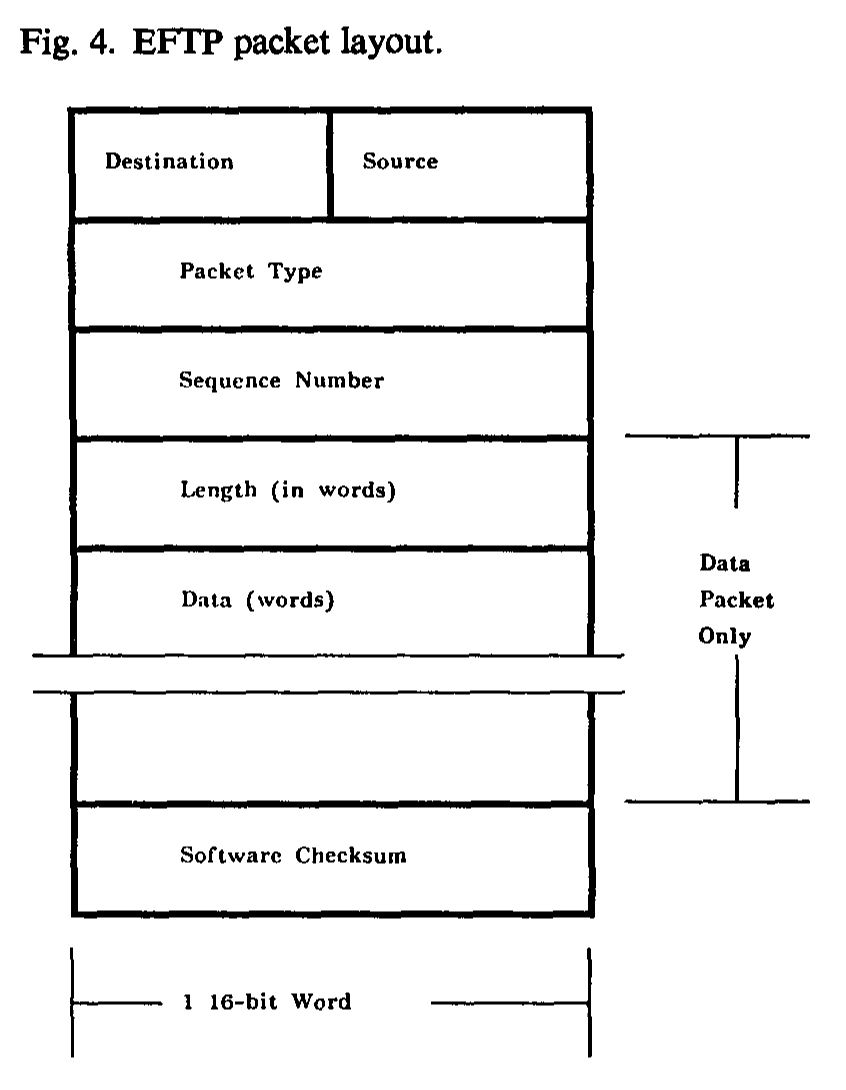
\includegraphics[trim =0mm 0mm 0mm 0mm, clip, width=6cm]{Ethernet-Fig-4.png}    \caption{Ethernet-Fig-4.png} \end{figure}

% This is what ChatGPT came up with  
%\begin{figure}[ht]
%  \centering
%  % Shrink text slightly and widen the boxes
%  {\scriptsize
%    \begin{bytefield}[bitwidth=2em]{32}
%      % Label bit columns 0-15 and 16-31
%      \bitheader{0-15,16-31} \\
%
%      % First row: 16 bits for Destination, 16 bits for Source
%      \bitbox{16}{\textbf{Destination}} & \bitbox{16}{\textbf{Source}} \\[0.5em]
%
%      % Next rows occupy the entire 32-bit width
%      \bitbox{32}{\textbf{Packet Type}} \\[0.5em]
%      \bitbox{32}{\textbf{Sequence Number}} \\[0.5em]
%      \bitbox{32}{\textbf{Length (in words)}} \\[0.5em]
%
%      % Annotate “Data Packet Only” on the right edge
%      \begin{rightwordgroup}{\scriptsize Data Packet Only}
%        \bitbox{32}{\textbf{Data (words)}}
%      \end{rightwordgroup}\\[0.5em]
%
%      \bitbox{32}{\textbf{Software Checksum}}
%    \end{bytefield}
%  }
%  \caption{EFTP packet layout using the \texttt{bytefield} package.}
%  \label{fig:eftp-packet}
%\end{figure}
%
%\begin{figure}[ht]
%  \centering
%  % A minipage that takes half the text width
%  \begin{minipage}{0.5\textwidth}
%    \centering
%    % Shrink text and reduce the bitwidth
%    {\scriptsize
%      \begin{bytefield}[bitwidth=1em]{32}
%        \bitheader{0-15,16-31} \\
%        \bitbox{16}{\textbf{Destination}} & \bitbox{16}{\textbf{Source}} \\[0.5em]
%        \bitbox{32}{\textbf{Packet Type}} \\[0.5em]
%        \bitbox{32}{\textbf{Sequence Number}} \\[0.5em]
%        \bitbox{32}{\textbf{Length (in words)}} \\[0.5em]
%        \begin{rightwordgroup}{\scriptsize Data Packet Only}
%          \bitbox{32}{\textbf{Data (words)}}
%        \end{rightwordgroup}\\[0.5em]
%        \bitbox{32}{\textbf{Software Checksum}}
%      \end{bytefield}
%    }
%    \caption{EFTP packet layout (compressed to half the page).}
%    \label{fig:eftp-packet}
%  \end{minipage}
%\end{figure}


%\begin{figure}[ht]
%  \centering
%  \begin{minipage}{0.5\textwidth}
%    \centering
%    % Slightly smaller text, and each row is 16 bits total.
%    {\scriptsize
%      \begin{bytefield}[bitwidth=2em]{16}
%        % Show the bit headers for 0--7 and 8--15
%        \bitheader{0-7,8-15}\\
%        % First row has two 8-bit fields side by side
%        \bitbox{8}{\textbf{Destination}} & \bitbox{8}{\textbf{Source}} \\[0.5em]
%
%        % Each subsequent field spans the full 16 bits
%        \bitbox{16}{\textbf{Packet Type}}         \\[0.5em]
%        \bitbox{16}{\textbf{Sequence Number}}     \\[0.5em]
%        \bitbox{16}{\textbf{Length (in words)}}   \\[0.5em]
%
%        % Rightwordgroup annotation for "Data Packet Only"
%        \begin{rightwordgroup}{\scriptsize Data Packet Only}
%          \bitbox{16}{\textbf{Data (words)}}
%        \end{rightwordgroup}\\[0.5em]
%
%        \bitbox{16}{\textbf{Software Checksum}}
%      \end{bytefield}
%    }
%    \caption{EFTP packet layout in a 16-bit‐wide diagram.}
%    \label{fig:eftp-packet-16bit}
%  \end{minipage}
%\end{figure}



\begin{figure}[ht]
  \centering
  \begin{minipage}{0.5\textwidth}
    \centering
    {\scriptsize
      % 16 bits wide
      \begin{bytefield}[bitwidth=1.5em]{16}
        \bitheader{0-7,8-15} \\

        \bitbox{8}{\textbf{Destination}} & \bitbox{8}{\textbf{Source}} \\[0.6em]
        \bitbox{16}{\textbf{Packet Type}}         \\[0.6em]
        \bitbox{16}{\textbf{Sequence Number}}     \\[0.6em]
        \bitbox{16}{\textbf{Length (in words)}}   \\[0.6em]

        % -- Data section with a wavy line to indicate variable length --
        \begin{rightwordgroup}{\footnotesize Data Packet Only}
          % First Data Word
          \bitbox{16}{\textbf{Data Word 1}} \\[-0.2em]

          % A 'wavy' row to show that many words can follow
          % Use \wordbox with partial lines around it
          \wordbox[lrt]{1}{%
            \centering
            \raisebox{-0.5ex}{\Huge$\sim\!\sim\!\sim$}%
          }\\[-0.2em]

          % Last Data Word shown
          \bitbox{16}{\textbf{Data Word N}} \\
        \end{rightwordgroup}\\[0.6em]

        \bitbox{16}{\textbf{Software Checksum}}

      \end{bytefield}
    }
    \caption{EFTP packet layout with a variable‐length “Data” field.}
    \label{fig:eftp-variable-length}
  \end{minipage}
\end{figure}



%% This is what ChatGPT came up with for Figure 3 in the Metcalfe + Boggs Paper

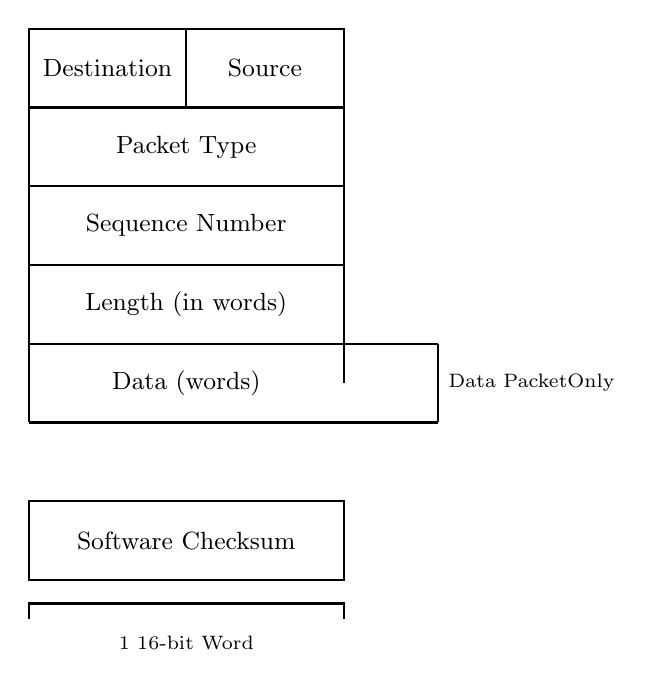
\begin{tikzpicture}[
  font=\sffamily,
  thick,
  % For quick coordinate adjustments, each "word" is 4 cm wide:
  x=4cm,
  % Each row is 1 cm high:
  y=1cm
]

% We will stack rectangles downward (negative y).
% The top left corner of the top row is (0,0).

% 1) Top row: Destination (left half), Source (right half)
\draw (0,0) rectangle (1,-1); % Entire top row is 1 "word" wide in x-coords
\draw (0.5,0) -- (0.5,-1);    % Subdivide into two half-words
% Labels:
\node[align=center, font=\small] at (0.25,-0.5) {Destination};
\node[align=center, font=\small] at (0.75,-0.5) {Source};

% 2) Packet Type row
\draw (0,-1) rectangle (1,-2);
\node[font=\small] at (0.5,-1.5) {Packet Type};

% 3) Sequence Number row
\draw (0,-2) rectangle (1,-3);
\node[font=\small] at (0.5,-2.5) {Sequence Number};

% 4) Length (in words) row
\draw (0,-3) rectangle (1,-4);
\node[font=\small] at (0.5,-3.5) {Length (in words)};

% 5) Data (words) area.
%   We'll show it as partially open at the bottom to suggest variable length.
%   Top line from y=-4 to y=-5, no bottom line to the next box.
\draw (0,-4) -- (1,-4) (0,-5) -- (1,-5); % horizontal lines
\draw (0,-4) -- (0,-5); % left vertical
\draw (1,-4) -- (1,-4.5); % partial right vertical
\node[font=\small] at (0.5,-4.5) {Data (words)};
% "Data Packet Only" bracket on the right
\draw (1,-4) -- ++(0.3,0) 
      (1,-5) -- ++(0.3,0);
\draw (1.3,-4) -- (1.3,-5);
\node[font=\scriptsize, right] at (1.3,-4.5) {Data Packet\\Only};

% 6) Software Checksum row (below data).
%   For simplicity, place it two rows below, i.e. from y=-6 to y=-7
\draw (0,-6) rectangle (1,-7);
\node[font=\small] at (0.5,-6.5) {Software Checksum};
% Optionally draw a horizontal line at y=-5 or -5.5 to “close” the data region:
% \draw (0,-5.5) -- (1,-5.5);

% “1 16-bit Word” bracket at the very bottom
%   We draw a bracket from x=0 to x=1 at y=-7.5, then label underneath
\draw (0,-7.5) -- (0,-7.3) -- (1,-7.3) -- (1,-7.5);
\node[font=\scriptsize] at (0.5,-7.8) {1 16-bit Word};

\end{tikzpicture}


 
 
 \section*{TABLE 1}

 
%!TEX root =Metcalfe+Boggs.tex
% This is what ChatGPT came up with for Table 1 3 in the Metcalfe + Boggs Paper

\begin{table}[ht]
\centering \tiny % \small
\caption*{Table 1. Ethernet Efficiency}
%\label{tab:ethernet-efficiency}
\begin{tabular}{c|cccc}
\hline
\textbf{Q} & \textbf{P = 4096} & \textbf{P = 1024} & \textbf{P = 512} & \textbf{P = 48} \\
\hline
1   & 1.0000 & 1.0000 & 1.0000 & 1.0000 \\
2   & 0.9884 & 0.9552 & 0.9143 & 0.5000 \\
3   & 0.9857 & 0.9447 & 0.8951 & 0.4444 \\
4   & 0.9842 & 0.9396 & 0.8862 & 0.4219 \\
5   & 0.9834 & 0.9367 & 0.8810 & 0.4096 \\
10  & 0.9818 & 0.9310 & 0.8709 & 0.3874 \\
32  & 0.9807 & 0.9272 & 0.8642 & 0.3737 \\
64  & 0.9805 & 0.9263 & 0.8627 & 0.3708 \\
128 & 0.9804 & 0.9259 & 0.8620 & 0.3693 \\
256 & 0.9803 & 0.9257 & 0.8616 & 0.3686 \\
\hline
\end{tabular}
\end{table}

%%[[Graph from Above Table  -- THIS IS NOT IN ORIGINAL PAPER]]
%
%\begin{figure}[ht]
%    \centering \small
%    \begin{tikzpicture}
%    \begin{axis}[
%        width=0.5\textwidth,
%        xlabel={\(\displaystyle Q\)},
%        ylabel={Efficiency},
%        xmin=0, xmax=260,
%        ymin=0.3, ymax=1.05,
%        legend pos=south west,
%        grid=both
%    ]
%    
%    %-- P = 4096
%    \addplot[
%        mark=o,
%        blue
%    ]
%    coordinates {
%        (1,1.0000)
%        (2,0.9884)
%        (3,0.9857)
%        (4,0.9842)
%        (5,0.9834)
%        (10,0.9818)
%        (32,0.9807)
%        (64,0.9805)
%        (128,0.9804)
%        (256,0.9803)
%    };
%    \addlegendentry{P = 4096}
%    
%    %-- P = 1024
%    \addplot[
%        mark=square,
%        red
%    ]
%    coordinates {
%        (1,1.0000)
%        (2,0.9552)
%        (3,0.9447)
%        (4,0.9396)
%        (5,0.9367)
%        (10,0.9310)
%        (32,0.9272)
%        (64,0.9263)
%        (128,0.9259)
%        (256,0.9257)
%    };
%    \addlegendentry{P = 1024}
%    
%    %-- P = 512
%    \addplot[
%        mark=triangle,
%        brown
%    ]
%    coordinates {
%        (1,1.0000)
%        (2,0.9143)
%        (3,0.8951)
%        (4,0.8862)
%        (5,0.8810)
%        (10,0.8709)
%        (32,0.8642)
%        (64,0.8627)
%        (128,0.8620)
%        (256,0.8616)
%    };
%    \addlegendentry{P = 512}
%    
%    %-- P = 48
%    \addplot[
%        mark=*,
%        green!60!black
%    ]
%    coordinates {
%        (1,1.0000)
%        (2,0.5000)
%        (3,0.4444)
%        (4,0.4219)
%        (5,0.4096)
%        (10,0.3874)
%        (32,0.3737)
%        (64,0.3708)
%        (128,0.3693)
%        (256,0.3686)
%    };
%    \addlegendentry{P = 48}
%    
%    \end{axis}
%    \end{tikzpicture}
%%    \caption{Ethernet Efficiency vs.\ Q for Different Packet Sizes \(P\)}
%    \label{fig:ethernet-efficiency-plot}
%\end{figure}


%!TEX root =../Metcalfe+Boggs.tex

%[[Graph from Above Table  -- THIS IS NOT IN ORIGINAL PAPER]]

\begin{figure}[ht]
    \centering \small 
       \caption*{\small Graph of Ethernet Efficiency [Not in Original Paper]}
    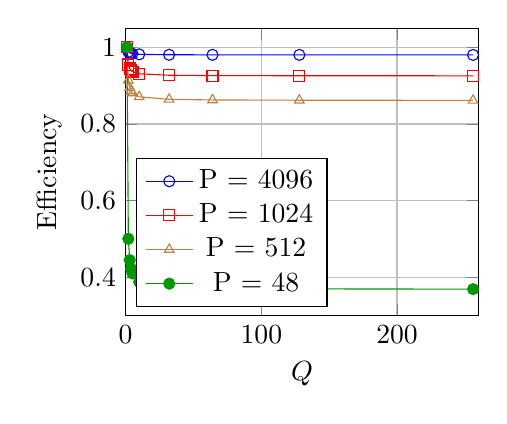
\begin{tikzpicture}
    \begin{axis}[
        width=0.5\textwidth,
        xlabel={\(\displaystyle Q\)},
        ylabel={Efficiency},
        xmin=0, xmax=260,
        ymin=0.3, ymax=1.05,
        legend pos=south west,
        grid=both
    ]
    
    %-- P = 4096
    \addplot[
        mark=o,
        blue
    ]
    coordinates {
        (1,1.0000)
        (2,0.9884)
        (3,0.9857)
        (4,0.9842)
        (5,0.9834)
        (10,0.9818)
        (32,0.9807)
        (64,0.9805)
        (128,0.9804)
        (256,0.9803)
    };
    \addlegendentry{P = 4096}
    
    %-- P = 1024
    \addplot[
        mark=square,
        red
    ]
    coordinates {
        (1,1.0000)
        (2,0.9552)
        (3,0.9447)
        (4,0.9396)
        (5,0.9367)
        (10,0.9310)
        (32,0.9272)
        (64,0.9263)
        (128,0.9259)
        (256,0.9257)
    };
    \addlegendentry{P = 1024}
    
    %-- P = 512
    \addplot[
        mark=triangle,
        brown
    ]
    coordinates {
        (1,1.0000)
        (2,0.9143)
        (3,0.8951)
        (4,0.8862)
        (5,0.8810)
        (10,0.8709)
        (32,0.8642)
        (64,0.8627)
        (128,0.8620)
        (256,0.8616)
    };
    \addlegendentry{P = 512}
    
    %-- P = 48
    \addplot[
        mark=*,
        green!60!black
    ]
    coordinates {
        (1,1.0000)
        (2,0.5000)
        (3,0.4444)
        (4,0.4219)
        (5,0.4096)
        (10,0.3874)
        (32,0.3737)
        (64,0.3708)
        (128,0.3693)
        (256,0.3686)
    };
    \addlegendentry{P = 48}
    
    \end{axis}
    \end{tikzpicture}
%    \caption*{\small Ethernet Efficiency vs.$Q$ for Different Packet Sizes $P$}
    \label{fig:ethernet-efficiency-plot}
\end{figure}


\end{document}
  
 

\end{document}  